\documentclass{article}
\usepackage[utf8]{inputenc}
\usepackage[T1]{fontenc}
\usepackage{amsmath}
\usepackage{amssymb}
\usepackage{enumitem}
\usepackage{geometry}
\usepackage{fancyhdr}
%\usepackage[hyphens]{url}
\usepackage{graphicx}
\usepackage{vwcol} 
\usepackage{multicol}
\usepackage{nopageno}
\usepackage{fontawesome}
\usepackage{setspace}
\usepackage{helvet}
 \fontfamily{phv}\selectfont
\usepackage[compact]{titlesec}
\titlespacing{\section}{0pt}{0pt}{0pt}
\usepackage{xcolor}
\usepackage[breaklinks=true]{hyperref}
%\usepackage{breakurl}
\hypersetup{
colorlinks = true,
linkcolor = blue,
urlcolor = red
}
\geometry{
 a4paper,
 total={190mm,257mm},
 left=10mm,
 top=40mm,
 headheight=30mm
 }

\urlstyle{same}

\pagestyle{fancy}
\fancyhf{}
\rhead{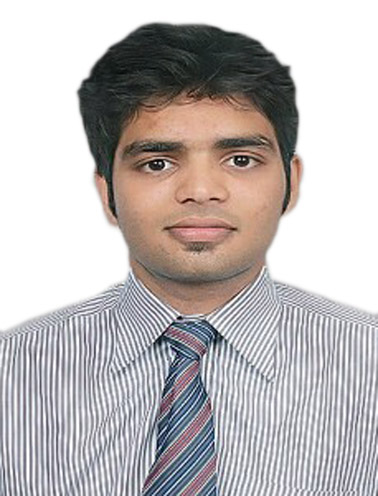
\includegraphics[width=2.5cm, height=3cm]{Photo.jpg}}
\chead{\LARGE {\uppercase{\textbf{Prahlad Amudan}} }}



\begin{document}
\begin{multicols}{2}
%\begin{vwcol}[widths={0.4,0.6},
%sep=.8cm, justify=flush,rule=0pt,indent=1em]
%[
%\section{\LARGE{\uppercase{\textbf{Prahlad Amudan}}}}
%All human things are subject to decay. And when fate summons, Monarchs must obey.
%]


\section*{\large{\uppercase{contact:}}}
%\vspace{3pt}
\flushleft{

\faPhone \hspace{1mm} Phone: +919833004100\\
\faEnvelopeO \hspace{1mm} {\color{red}\underline{\href{mailto:prahlad2001a@gmail.com}{prahlad2001a@gmail.com}}} \\
\faHome \hspace{1mm} 2nd Floor,Brahma Niwas,Near Pangong Tso Lake, Chembur,Mumbai-400089 \\ 
\faLinkedin\hspace{1mm}  LinkedIn: {\color{red}\underline{\href{https://www.linkedin.com/in/Prahlad-Amudan-060598155}{https://www.linkedin.com/in/Prahlad-Amudan-060598155}}}\\
\faGithub\hspace{1mm} Github: {\color{red}\underline{\href{mailto:prahlad2001a@gmail.com}{www.github.com/in/Prahlad-Amudan}}}
}

\vspace{10pt}
\section*{\large{\uppercase{education:}}}

%\vspace{3pt}

\flushleft{

{\textbf{Veermata Jijabai Technological Institute(VJTI)}}\\{\textbf{CGPA}}: 10 \hspace{30mm} {\textbf{Percentage}}: - \\ {\textbf{From}}: 14/08/2019 - 14/08/2023\\
{\textbf{Course Work}} : Thermodynamics, Fluid Mechanics, Coding, Mechatronics, Entreprenuership,Computer Programming, Basic Electrical Engineering, Elements of Mechanical Engineering, Mechanics, Graphics.\\


{\textbf{\underline{Professional Associations}}}:
\begin{itemize}[noitemsep,nolistsep]
	
	\item Member of Entrepreneurship-cell VJTI
	\item Member of American Society of Mechanical Engineers(ASME)(VJTI)
	\item Member of Institute of Electrical and Electronics Engineers(IEEE)(VJTI)
	
\end{itemize}
\vspace{3pt}
{\textbf{South Indian Education Society(SIES)}} \\
\textbf{CGPA}: -  \hspace{3cm}      \textbf{Percentage}: 91\% \\
\textbf{From}: 15/06/2017 - 20/03/2019 \\   
\textbf{Course Work}:
Studied For JEE Mains and Advanced and various other competitive exams \\
{\textbf{\underline{Professional Associations}}}:
\begin{itemize}[noitemsep,nolistsep]
	\item Member of College's event organiser's team
  
\end{itemize} 


}
\vspace{5pt}


\section*{\large{\uppercase{Hobbies:}}}

%\vspace{3pt}
\begin{flushleft}
\begin{itemize}[noitemsep,nolistsep]
	\item Reading Different kinds of books, Programming, listening to classical Indian music
	\item Blogging, Volunteering, Traveling, Art, Design, Music, Reading, Video Gaming.
\end{itemize}
\end{flushleft}
\vspace{5pt}
\columnbreak

\section*{\large{\uppercase{objective:}}}

%\vspace{3pt}
\begin{flushleft}
The decision about what to put into your paragraphs begins with the germination of a seed of ideas; this germination process is better known as brainstorming. 
\end{flushleft}

\vspace{3pt}
\section*{\large{\uppercase{Skills:}}}

%\vspace{3pt}
\begin{flushleft}
\begin{itemize}[noitemsep,nolistsep]
	\item AutoCAD, Solidworks, AutoCAD Mechanical, Autodesk Inventor
	\item Excel, C++, HTML, Javascript, Python
	\item Management, Leadership, Organization, Public Speaking, Problem-solving, Teamwork
\end{itemize}
\end{flushleft}
\vspace{5pt}



\section*{\large{\uppercase{projects:}}}

%\vspace{3pt}

\begin{enumerate}[noitemsep,nolistsep]
	\item {\textbf{Resume Builder}}\\
	\hfill {\textbf{From}}: May-20 {\textbf{To}} July-20\\
	Piranhas rarely feed on large animals; they eat smaller fish and aquatic plants. When confronted with humans, piranhas first instinct is to flee, not attack. 
	\item {\textbf{Fan Controlled using Bluetooth}}\\
	\hfill {\textbf{From}}: Dec-19 {\textbf{To}} Mar-20\\
	Although most people consider piranhas to be quite dangerous, they are, for the most part, entirely harmless. Piranhas rarely feed on large animals; they eat smaller fish and aquatic plants.
\end{enumerate}

\vspace{5pt}

\section*{\large{\uppercase{Internship:}}}

%\vspace{3pt}

\begin{enumerate}[noitemsep,nolistsep]
	\item {\textbf{Internship at Google}}\\
	\hfill {\textbf{From}}: Mar-20 {\textbf{To}} May-20\\
	Developing writers can often benefit from examining an essay, a paragraph, or even a sentence to determine what makes it effective. On the following pages are several paragraphs for you to evaluate on your own, along with the Writing Center's explanation.
	\item {\textbf{Internship at Lockheed Martin}}\\
	\hfill {\textbf{From}}: May-20 {\textbf{To}} Nov-20\\
	 Scientists research has revealed that viruses are by far the most abundant life forms on Earth. There are a million times more viruses on the planet than stars in the universe. Viruses also harbor the majority of genetic diversity on Earth. 
\end{enumerate}

\vspace{5pt}

\section*{\large{\uppercase{achievements:}}}

\vspace{0pt}
\flushleft{
\begin{itemize}[noitemsep,nolistsep]
	\item Was a part of State level football team
	\item Won many national and international level olympiads
	\item Won 3rd Prize in National level Drawing competition
\end{itemize}
}
\vspace{5pt}

%\end{vwcol}
\end{multicols}
\end{document}
